\documentclass[12pt,a4paper]{article}
\usepackage{ctex}
\usepackage{amsmath,amscd,amsbsy,amssymb,latexsym,url,bm,amsthm}
\usepackage{epsfig,graphicx,subfigure}
\usepackage{enumitem,balance}
\usepackage{wrapfig}
\usepackage{listings}
\usepackage{mathrsfs,euscript}
\usepackage[usenames]{xcolor}
\usepackage{hyperref}
\usepackage[vlined,ruled,linesnumbered]{algorithm2e}
\usepackage{array}
\hypersetup{colorlinks=true,linkcolor=black}

\lstset{
    breaklines,
    basicstyle          =   \ttfamily,
    commentstyle        =   \rmfamily\itshape,
    stringstyle         =   \ttfamily,
    flexiblecolumns,
    numbers             =   left,
    showspaces          =   false,
    numberstyle         =   \zihao{-5}\ttfamily,
    showstringspaces    =   false,
    captionpos          =   t,
    frame               =   lrtb,
}

\newtheorem{theorem}{Theorem}
\newtheorem{lemma}[theorem]{Lemma}
\newtheorem{proposition}[theorem]{Proposition}
\newtheorem{corollary}[theorem]{Corollary}
\newtheorem{exercise}{Exercise}
\newtheorem*{solution}{Solution}
\newtheorem{definition}{Definition}
\theoremstyle{definition}

\renewcommand{\thefootnote}{\fnsymbol{footnote}}

\newcommand{\postscript}[2]
 {\setlength{\epsfxsize}{#2\hsize}
  \centerline{\epsfbox{#1}}}

\renewcommand{\baselinestretch}{1.0}

\setlength{\oddsidemargin}{-0.365in}
\setlength{\evensidemargin}{-0.365in}
\setlength{\topmargin}{-0.3in}
\setlength{\headheight}{0in}
\setlength{\headsep}{0in}
\setlength{\textheight}{10.1in}
\setlength{\textwidth}{7in}
\makeatletter \renewenvironment{proof}[1][Proof] {\par\pushQED{\qed}\normalfont\topsep6\p@\@plus6\p@\relax\trivlist\item[\hskip\labelsep\bfseries#1\@addpunct{.}]\ignorespaces}{\popQED\endtrivlist\@endpefalse} \makeatother
\makeatletter
\renewenvironment{solution}[1][Solution] {\par\pushQED{\qed}\normalfont\topsep6\p@\@plus6\p@\relax\trivlist\item[\hskip\labelsep\bfseries#1\@addpunct{.}]\ignorespaces}{\popQED\endtrivlist\@endpefalse} \makeatother

\begin{document}
\noindent

%========================================================================
\noindent\framebox[\linewidth]{\shortstack[c]{
\Large{\textbf{Lab09-Network Flow}}\vspace{1mm}\\
CS214-Algorithm and Complexity, Xiaofeng Gao, Spring 2020.}}
\begin{center}
\footnotesize{\color{red}$*$ If there is any problem, please contact TA Shuodian Yu. }

\footnotesize{\color{blue}$*$ Name:Hongjie Fang  \quad Student ID:518030910150 \quad Email: galaxies@sjtu.edu.cn}
\end{center}
\begin{enumerate}
\item Given a weighted directed graph $G (V, E)$ and its corresponding weight matrix $W=(w_{ij})_{n \times n}$ and shortest path matrix $D=(d_{ij})_{n \times n}$, where $w_{ij}$ is the weight of edge $(v_i, v_j)$ and $d_{ij}$ is the weight of a shortest path from pairwise vertex $v_i$ to $v_j$. Now, assume the weight of a particular edge $(v_a, v_b)$ is decreased from $w_{ab}$ to $w'_{ab}$. Design an algorithm to update matrix $D$ with respect to this change, whose time complexity should be no larger than $O(n^2)$. Describe your design first and write down your algorithm in the form of pseudo-code.
    \begin{solution} We assume that there is \underline{no negative cycle} in both the original graph $G$ and the new graph after updating. Here is my algorithm design.

        For every pair of vertices $(v_x, v_y)$, check if path $v_x \rightsquigarrow v_a \rightarrow v_b \rightsquigarrow v_y$ is shorter than the current shortest path $v_x \rightsquigarrow v_y$ in new graph. If so, then update the shortest path $d_{xy}$ to $d_{xa} + w'_{ab} + d_{by}$.

        \textbf{(Correctness Explanation)} First, there exists a shortest path from $v_x$ to $v_a$ that \underline{does not} \underline{contain edge $(v_a, v_b)$}. If not, then there must be at least one cycle containing edge $(v_a, v_b)$ in the shortest path from $v_x$ to $v_a$ because we visit $v_a$ at least twice. We can eliminate all the zero cycle in the shortest path from $v_x$ to $v_a$ first without changing the total weight of the shortest path, and at least one non-zero cycle containing $(v_a, v_b)$ must remain after the operation, or it will contradicts the premise that all the shortest path from $v_x$ to $v_a$ contains edge $(v_a, v_b)$. After that, we make the following discussions.
        \begin{itemize}
        \item If it is a negative cycle, then it contradicts the assumption that there is no negative cycle;
        \item If it is a positive cycle, then we can eliminate it to form a shorter path from $v_x$ to $v_a$, which contradicts the premise that it is a shortest path from $x$ to $a$.
        \end{itemize}
        In summary, there exists a shortest path from $v_x$ to $v_a$ that does not contain edge $(v_a, v_b)$. Similarly, there exists a shortest path from $v_b$ to $v_y$ that does not contain $(v_a, v_b)$. Therefore, {\color{blue}the weight change of edge $(v_a, v_b)$ does not affect the shortest path from $v_x$ to $v_a$ and the shortest path from $v_b$ to $v_y$}, which means the shortest paths $d_{\cdot a}$ whose destinations are $v_a$ and the shortest paths $d_{b \cdot}$ whose sources are $v_b$ must remain the same after the weight change.

        Since the weight of $(v_a, v_b)$ is decreased, we can check if path $v_x \rightsquigarrow v_a \rightarrow v_b \rightsquigarrow v_y$ is shorter than the current shortest path. These two parts $v_x \rightsquigarrow v_a$ and $v_b \rightsquigarrow v_y$ are not influenced by the weight change of edge $(v_a, v_b)$.
        Thus, for every original shortest path from $v_x$ to $v_y$:
        \begin{itemize}
        \item If the weight change does not affect it, then $d_{ij}$ will not change in our algorithm;
        \item If it has the edge $(v_a, v_b)$, then $d_{ij}$ is bound to be updated because the new weight of the shortest path $d_{xa} + w'_{ab} + d_{by}$ is less than the old one $d_{xy} = d_{xa} + w_{ab} + d_{by}$;
        \item If it does not have the edge $(v_a, v_b)$ but after weight change the new shortest path should contain $(v_a, v_b)$, then it will also be taken into consideration because we check the path $v_x \rightsquigarrow v_a \rightarrow v_b \rightsquigarrow v_y$. Since the weight change does not affect $v_x \rightsquigarrow v_a$ and $v_b \rightsquigarrow v_y$, then path $v_x \rightsquigarrow v_a \rightarrow v_b \rightsquigarrow v_y$ must be the shortest path from $v_x$ to $v_y$ passing edge $(v_a, v_b)$. Therefore, we must update the shortest path from $v_x$ to $v_y$ in our algorithm.
        \end{itemize}

        In summary, our algorithm will update the shortest path matrix correctly.
        \clearpage
        \textbf{(Time Complexity Analysis)} We check every pair of vertices once, and the time complexity of the possible updating process is $O(1)$. There are $n^2$ pairs of vertices in total. Therefore, the total time complexity of the algorithm is $O(n^2)$.

        \textbf{(Pseudo-Code)} The pseudo-code of the algorithm is as follows.
        \begin{center}
        \begin{minipage}[t]{0.8\textwidth}
        \begin{algorithm}[H]
            \KwIn{A directed graph $G (V, E)$; the weight matrix $W = (w_{ij})_{n \times n}$ and the shortest path matrix $D = (d_{ij})_{n\times n}$ of graph $G$; the particular edge $(v_a, v_b)$ and its new weight $w'_{ab}$.}
            \KwOut{The new shortest path matrix $D = (d_{ij})_{n \times n}$ after updating with respect to the weight change of $(v_a, v_b)$.}

            \BlankLine
            \caption{Shortest Path Matrix Update Algorithm}
            \label{alg1}

            \ForEach{$v_x \in V$} {
                \ForEach{$v_y \in V$} {
                    \If{$d_{xa} + w'_{ab} + d_{by} < d_{xy}$} {
                        $d_{xy} \leftarrow d_{xa} + w'_{ab} + d_{by}$;
                    }
                }
            }

            \Return{$(d_{ij})_{n \times n}$};
        \end{algorithm}
        \end{minipage}
        \end{center}

    \end{solution}
    \clearpage

	\item Given a directed graph $G$, whose vertices and edges information are introduced in data file ``SCC.in''. Please find its number of Strongly Connected Components with respect to the following subquestions.
    \begin{enumerate}
    	\item Read the code and explanations of the provided C/C++ source code ``SCC.cpp'', and try to complete this implementation.
    	\item Visualize the above selected Strongly Connected Components for this graph $G$. Use the $Gephi$ or other software you preferred to draw the graph. {\color{blue}(If you feel that the data provided in ``SCC.in'' is not beautiful, you can also generate your own data with more vertices and edges than $G$ and draw an additional graph. Notice that results of your visualization will be taken into the consideration of Best Lab.)}

    \end{enumerate}
    \begin{solution} Here is the answers to each sub-question.
    \begin{enumerate}
    \item I use two different algorithms to compute the number of the strongly connected components in the graph $G$, and \underline{both of them output $666$ for the given input graph ``SCC.in''}, which means there are $666$ strongly connected components in the graph $G$.

        The first algorithm is \textbf{the Kosaraju algorithm}, which we have learnt in the course. The main source code of this algorithm is as follows. You can also refer to \href{code/SCC.cpp}{code/SCC.cpp} for full implementation. \underline{You may need to open the C++11 switch using \texttt{-std=c++11}}.
\begin{lstlisting}[language=C++]
void dfs(const vector < vector <int> > &E, int x, vector <int> &dfn, vector <int> &out, int &idx) {
  dfn[x] = ++idx;
  for (auto &dest: E[x])
    if (! dfn[dest]) dfs(E, dest, dfn, out, idx);
  out[x] = ++idx;
}

int SCC (int n, vector < pair <int, int> > &edge) {
  vector < vector <int> > E, Er;
  vector <int> dfn, out;
  vector <int> order;
  int idx, scc;

  E.resize(n);
  Er.resize(n);
  dfn.resize(n);
  out.resize(n);
  order.resize(n << 1);

  for (auto &edge_list: E) edge_list.clear();
  for (auto &edge_list: Er) edge_list.clear();

  for (auto &e: edge) {
    E[e.first].push_back(e.second);
    Er[e.second].push_back(e.first);
  }

  idx = 0;
  for (auto &d: dfn) d = 0;
  for (int i = 0; i < n; ++ i)
    if(! dfn[i]) dfs(Er, i, dfn, out, idx);

  for (auto &o: order) o = -1;
  for (int i = 0; i < n; ++ i) order[out[i] - 1] = i;

  scc = 0;
  idx = 0;
  for (auto &d: dfn) d = 0;
  for (int i = (n << 1) - 1; ~i; -- i)
    if(order[i] != -1 && ! dfn[order[i]]) {
      ++ scc;
      dfs(E, order[i], dfn, out, idx);
    }
  return scc;
}
\end{lstlisting}

        The second algorithm is \textbf{the Tarjan algorithm}. The main source code of this algorithm is as follows. You can also refer to \href{code/SCC-tarjan.cpp}{code/SCC-tarjan.cpp} for full implementation. \underline{You may need to open the C++11 switch using \texttt{-std=c++11}}.
\begin{lstlisting}
void tarjan(vector < vector <int> > &E, int x, vector <int> &dfn, vector <int> &low, vector <int> &instack, stack <int> &sta, int &idx, int &scc) {
  dfn[x] = low[x] = ++idx;
  sta.push(x);
  instack[x] = 1;

  for (auto &dest: E[x]) {
    if(! dfn[dest]) {
      tarjan(E, dest, dfn, low, instack, sta, idx, scc);
      low[x] = min(low[dest], low[x]);
    } else if (instack[dest]) low[x] = min(low[x], dfn[dest]);
  }

  if(dfn[x] == low[x]) {
    ++ scc;
    while(true) {
      int y = sta.top();
      sta.pop(); instack[y] = 0;
      if (y == x) break;
    }
  }
}

int SCC (int n, vector < pair <int, int> > &edge) {
  vector < vector <int> > E;
  vector <int> dfn, low;
  vector <int> instack;
  stack <int> sta;
  int idx, scc;

  E.resize(n);
  dfn.resize(n);
  low.resize(n);
  instack.resize(n);
  while(!sta.empty()) sta.pop();

  for (auto &edge_list: E) edge_list.clear();

  for (auto &e: edge)
    E[e.first].push_back(e.second);

  scc = 0;
  idx = 0;
  for (auto &d: dfn) d = 0;
  for (auto &in: instack) in = 0;
  for (int i = 0; i < n; ++ i)
    if(! dfn[i]) tarjan(E, i, dfn, low, instack, sta, idx, scc);

  return scc;
}
\end{lstlisting}
        \item If we \underline{regard each strongly connected component as a meta-node}, we can use Gephi to draw the following picture of the graph (Fig.~\ref{fig2-1}).
\begin{figure}[htbp]
  \centering
  % Requires \usepackage{graphicx}
  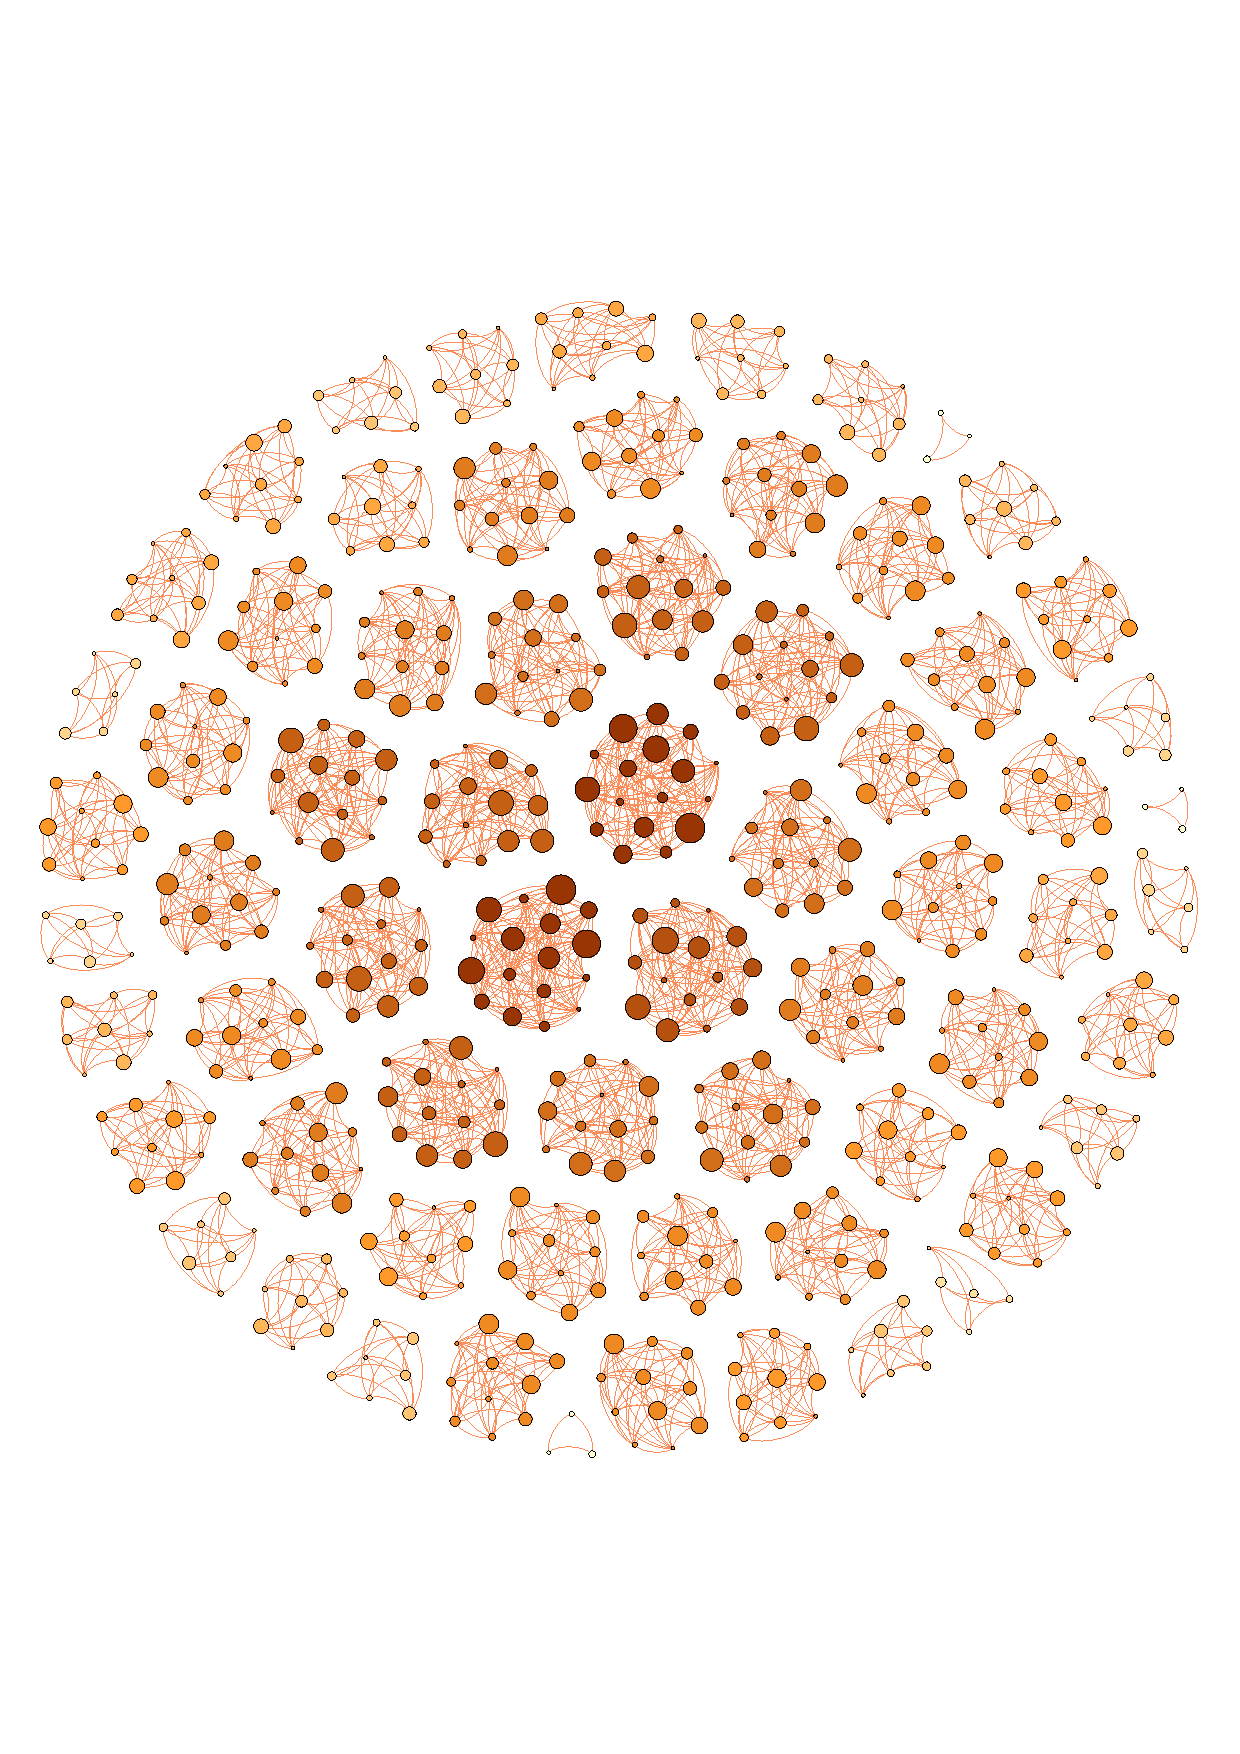
\includegraphics[width=3.2in]{pics/prob2-1.pdf}\\
  \caption{The visualization of the graph}\label{fig2-1}
\end{figure}
    \clearpage
    I generate a graph with $100000$ vertices and $601999$ edges myself, and the data is in the \href{code/newSCC.in}{code/newSCC.in}. The visualization of the newly generated graph is as follows. (Fig.~\ref{fig2-2}).
\begin{figure}[htbp]
  \centering
  % Requires \usepackage{graphicx}
  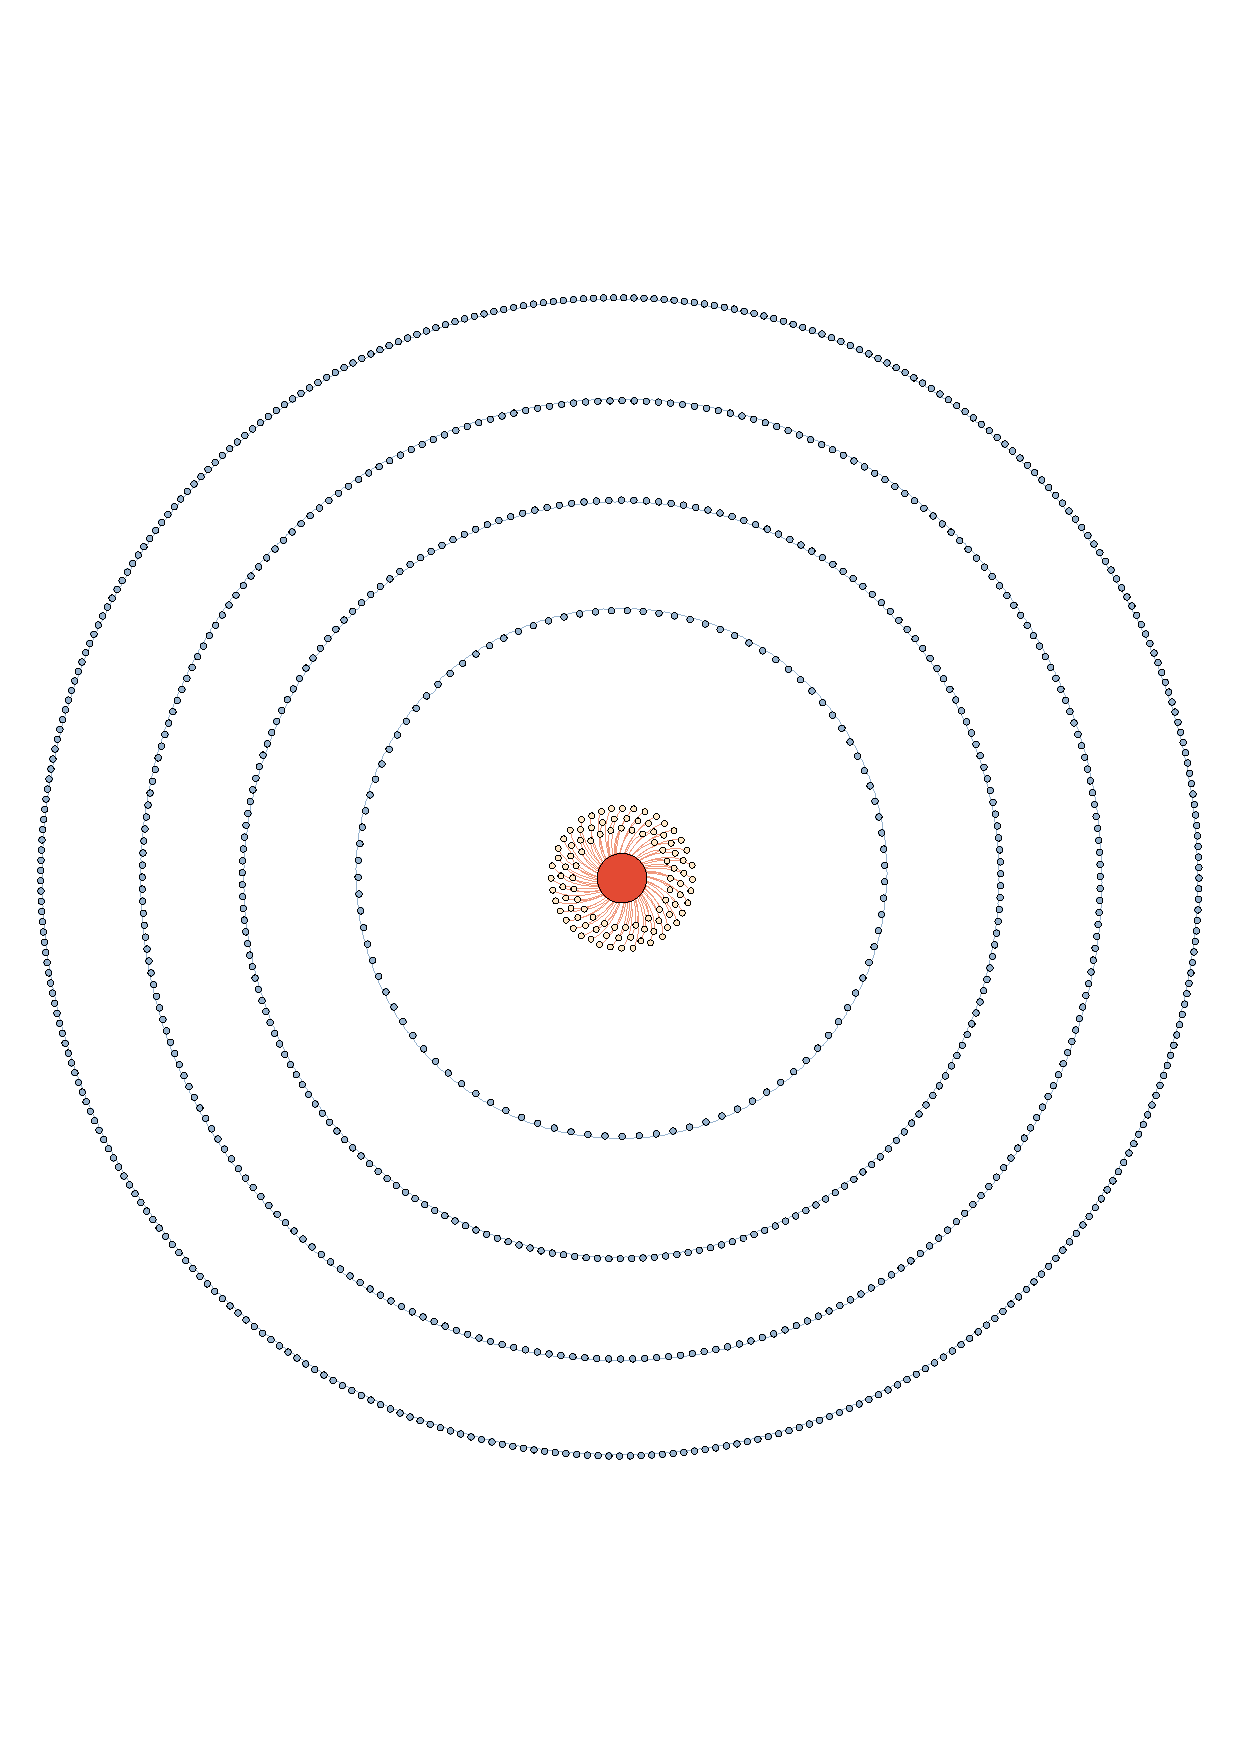
\includegraphics[width=5in]{pics/prob2-2.pdf}\\
  \caption{The visualization of the newly generated graph}\label{fig2-2}
\end{figure}
    \end{enumerate}
    \end{solution}

    \clearpage
	\item The \textbf{Minimum Cost Maximum Flow} problem (MCMF) is an optimization problem to find the cheapest possible way of sending the maximum amount of flow through a flow network. That is, in a flow network $G = (V, E)$ with a source $s\in V$ and a sink $t\in V$, where each edge $(u, v)\in E$ has a capacity $c(u,v) > 0$ and a cost $a(u,v) \ge 0$, find a maximum $s\text{-}t$ flow $f$ over all edges ($f(u, v) \ge 0)$, such that the total cost of $\sum_{(u, v) \in E} a(u, v) \cdot f(u, v)$ is minimized.

A common greedy approach to solve the MCMF problem can be described as follows: We can modify Ford-Fulkerson algorithm, where each time we choose the least cost path from $s$ to $t$. To do this correctly, when we add a back-edge to some edge $e$ into the residual graph, we give it a cost of $-a(e)$, representing that we get our money back if we undo the flow on it.

Note that such procedure may create a residual graph with negative-weight edges, which is not suitable for Dijkstra's Algorithm. However, motivated by Johnson's Algorithm, we can reweight the edge cost with vertex labels and convert the weight non-negative again.

Please prove the correctness of such greedy approach and implement this algorithm in C/C++. The file \emph{MCMF.in} is a test case, where the first line contains four graph parameters $n$, $m$, $s$, $t$, and the rest $m$ lines exhibit the information of $m$ edges. Each line contains four integers: $u_i$, $v_i$, $c_i$, $a_i$, denoting that there is an edge from $u_i$ to $v_i$ with capacity $c_i$ and cost $a_i$. {\color{blue}(Your source code should be named as \emph{MCMF.cpp} and output the maximum flow and minimum cost of this test case.)}

\begin{center}
\fbox{
\begin{minipage}[t]{0.3\textwidth}
\textbf{Sample Input:}
	
	4 5 4 3 \\ 4 2 30 2 \\ 4 3 20 3 \\ 2 3 20 1 \\ 2 1 30 9 \\ 1 3 40 5
\end{minipage}
\begin{minipage}[t]{0.3\textwidth}
\textbf{Sample Output: }
	
	50 280
\end{minipage}}
\end{center}
\hspace{1cm}
    \begin{definition}
    Let $a \rightarrow b$ denote an edge from $a$ to $b$; let $a \stackrel{F}{\rightarrow} b$ denote an edge from $a$ to $b$ in flow $F$; let $a \stackrel{-F}{\rightarrow} b$ denote a back edge from $a$ to $b$ in flow $F$; let $a \stackrel{r(F)}{\rightarrow} b$ denote an edge from $a$ to $b$ in the residual graph of flow $F$. A simple property is the edge $a \stackrel{-F}{\rightarrow} b$ can also be represented as $a \stackrel{r(F)}{\rightarrow} b$.
    \end{definition}
    \begin{definition}
    Let $a \rightsquigarrow b$ denote a path from $a$ to $b$; let $a \stackrel{F}{\rightsquigarrow} b$ denote a path from $a$ to $b$ in flow $F$; let $a \stackrel{-F}{\rightsquigarrow} b$ denote a path from $a$ to $b$ constructed by back edges in flow $F$. let $a \stackrel{r(F)}{\rightsquigarrow} b$ denote a path from $a$ to $b$ in the residual graph of flow $F$. A simple property is the path $a \stackrel{-F}{\rightsquigarrow} b$ can also be represented as $a \stackrel{r(F)}{\rightsquigarrow} b$.
    \end{definition}
    \begin{lemma}\label{lemma1}
    Given a value $v$, flow $F$ is the minimum cost flow among all the flows with value $v$ \textbf{if and only if} there is no negative cycle in the residual graph of flow $F$.
    \end{lemma}
    \begin{proof} We prove two directions of this lemma respectively as follows.
    \begin{itemize}
    \item \textbf{($\Longrightarrow$)} \textbf{(Contradiction)} If there exists at least one negative cycle in the residual graph of flow $F$ (Fig.~\ref{fig3-1}), then the negative cycle must contain at least one back edge, say $b \stackrel{-F}{\rightarrow} a$, since there is no negative weight edge in the initial graph. The negative cycle in the residual graph can be represented as $a \stackrel{r(F)}{\rightsquigarrow} b \stackrel{-F}{\rightarrow} a$. Then we can reduce the flow in edge $a \stackrel{F}{\rightarrow} b$ by $f\ (f > 0)$ and add the same amount of flow in path $a \stackrel{r(F)}{\rightsquigarrow} b$ to form a new flow $F'$. Since $a \stackrel{r(F)}{\rightsquigarrow} b \stackrel{-F}{\rightarrow} a$ is a negative cycle in the residual graph, we can make the following derivations.

        \begin{displaymath}
        \begin{aligned}
        cost(F') &= cost(F) - f \cdot cost(a \stackrel{F}{\rightarrow} b) + f \cdot cost(a \stackrel{r(F)}{\rightsquigarrow} b) \\
                 &= cost(F) + f \cdot cost(b \stackrel{-F}{\rightarrow} a) + f \cdot cost(a \stackrel{r(F)}{\rightsquigarrow} b) \\
                 &= cost(F) + f \cdot cost(a \stackrel{r(F)}{\rightsquigarrow} b \stackrel{-F}{\rightarrow} a) \\
                 &< cost(F)
        \end{aligned}
        \end{displaymath}

        Hence, flow $F'$ has the same value of flow $F$ but it costs less than flow $F$, which contradicts the premise that flow $F$ is the minimum cost flow of value $v$.
        \begin{figure}[htbp]
          \centering
          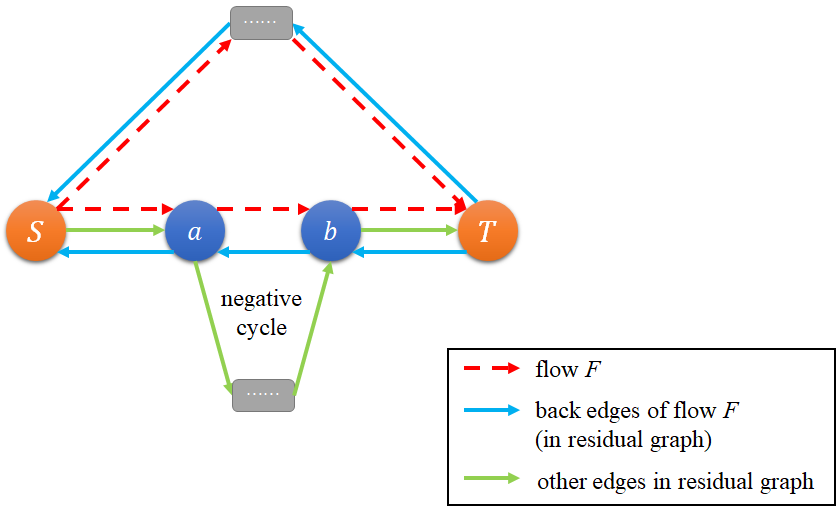
\includegraphics[width=3.1in]{pics/prob3-1.png}\\
          \caption{A negative cycle in the residual graph} \label{fig3-1}
        \end{figure}

    \item \textbf{($\Longleftarrow$)} \textbf{(Contradiction)} Suppose there is no negative cycle in the residual graph of flow $F$ but flow $F$ is not the minimum cost flow of value $v$. Then there exists another flow $F'$ with the same value, whose cost is less than flow $F$. According to the Flow Conservation Property and the Flow Value Lemma, the graph $F' - F$ is actually constructed by several cycles. At least one of the cycles has a negative weight because the cost of flow $F'$ is less than the cost of flow $F$ (Fig. \ref{fig3-2}). And the negative cycle in the graph $F'-F$ can be represented as $a \stackrel{F'}{\rightsquigarrow} b \stackrel{-F}{\rightsquigarrow} a$. Notice that the path $a \stackrel{F'}{\rightsquigarrow} b$ is also in the residual graph of flow $F$ since it is not in flow $F$. Therefore, there exists a negative cycle $a \stackrel{F'}{\rightsquigarrow} b \stackrel{-F}{\rightsquigarrow} a$ in the residual graph of flow $F$, which contradicts the premise.

        \begin{figure}[htbp]
          \centering
          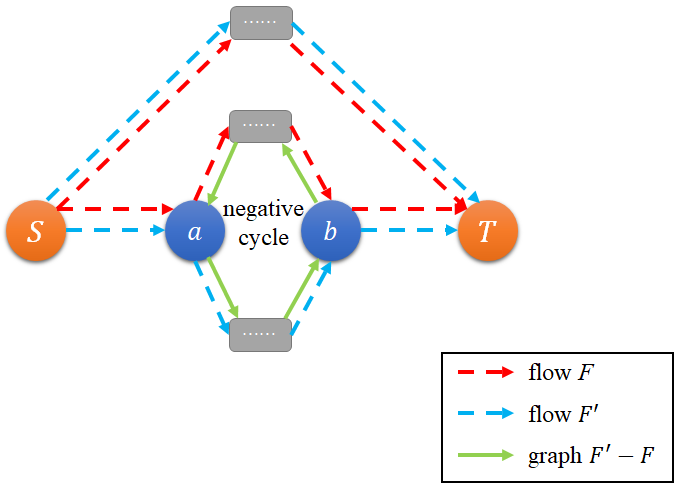
\includegraphics[width=2.6in]{pics/prob3-2.png}\\
          \caption{A negative cycle in graph $F' - F$} \label{fig3-2}
        \end{figure}
    \end{itemize}
    \end{proof}

    \begin{lemma}\label{lemma2}
    Our algorithm can terminates after finding a finite number of augmenting paths, and the result flow $F^*$ is the max flow of the flow network $G$.
    \end{lemma}
    \begin{proof}
    Our algorithm is actually \underline{a modified version of the Ford-Fulkerson Algorithm}. Using exact the same method of proof of the Ford-Fulkerson Algorithm, we can derive that if the algorithm terminates then the result flow $F^*$ is the max flow of the flow network $G$, and the algorithm terminates at most $val(F^*) \leq n \times C$ augmenting paths, where $C$ is the upper bound of the capacities of the edges.
    \end{proof}

    \begin{lemma}\label{lemma3}
    During the construction process of the max flow $F^*$ in our algorithm, there is no negative cycle in the residual graph of the current flow $F$.
    \end{lemma}

    \begin{proof}
    \textbf{(Induction)} In the beginning, our current flow $F$ is empty, so the residual graph of the current flow $F$ is actually the initial network $G$. And there is no negative cycle in $G$ according to the problem description.

    Suppose there is no negative cycle in the current flow $F$ after finding $n$ augmenting paths in our algorithm. We are going to prove there is still no negative cycle in flow $F'$ after adding an augmenting path based on flow $F$ in our algorithm.

    Flow $F'$ can be represented as $F \cup \{ s \stackrel{F'}{\rightsquigarrow} t\}$, where $s \stackrel{F'}{\rightsquigarrow} t$ is the new augmenting path. According to our algorithm, path $s \stackrel{F'}{\rightsquigarrow} t$ is the shortest path from $s$ to $t$. Suppose the residual graph of flow $F'$ contains a negative cycle (Fig.~\ref{fig3-3}). Then the negative cycle must contain some of the back edges in the new augmenting path $s \stackrel{F'}{\rightsquigarrow} t$, say $b \stackrel{-F'}{\rightsquigarrow} a$. Hence, path $s \stackrel{F'}{\rightsquigarrow} t$ can also be represented as $s \stackrel{F'}{\rightsquigarrow} a \stackrel{F'}{\rightsquigarrow} b \stackrel{F'}{\rightsquigarrow} t$, and the negative cycle can be represented as $a \stackrel{r(F')}{\rightsquigarrow} b \stackrel{-F'}{\rightsquigarrow} a$. Therefore, we can replace sub-path $a \stackrel{F'}{\rightsquigarrow} b$ with sub-path $a \stackrel{r(F')}{\rightsquigarrow} b$ to form a new path $s \stackrel{F'}{\rightsquigarrow} a \stackrel{r(F')}{\rightsquigarrow} b \stackrel{F'}{\rightsquigarrow} t$ from $s$ to $t$. Since $a \stackrel{r(F')}{\rightsquigarrow} b \stackrel{-F'}{\rightsquigarrow} a$ is a negative cycle, we can make the following derivations.
    \begin{displaymath}
    \begin{aligned}
    cost(s \stackrel{F'}{\rightsquigarrow} a \stackrel{r(F')}{\rightsquigarrow} b \stackrel{F'}{\rightsquigarrow} t) &= cost(s \stackrel{F'}{\rightsquigarrow} a \stackrel{F'}{\rightsquigarrow} b \stackrel{F'}{\rightsquigarrow} t) - cost(a \stackrel{F'}{\rightsquigarrow} b) + cost(a \stackrel{r(F')}{\rightsquigarrow} b) \\
    &= cost(s \stackrel{F'}{\rightsquigarrow} a \stackrel{F'}{\rightsquigarrow} b \stackrel{F'}{\rightsquigarrow} t) + cost(b \stackrel{-F'}{\rightsquigarrow} a) + cost(a \stackrel{r(F')}{\rightsquigarrow} b) \\
    &= cost(s \stackrel{F'}{\rightsquigarrow} a \stackrel{F'}{\rightsquigarrow} b \stackrel{F'}{\rightsquigarrow} t) + cost(a \stackrel{r(F')}{\rightsquigarrow} b \stackrel{-F'}{\rightsquigarrow} a) \\
    &< cost(s \stackrel{F'}{\rightsquigarrow} a \stackrel{F'}{\rightsquigarrow} b \stackrel{F'}{\rightsquigarrow} t)
    \end{aligned}
    \end{displaymath}
    \begin{figure}[htbp]
      \centering
      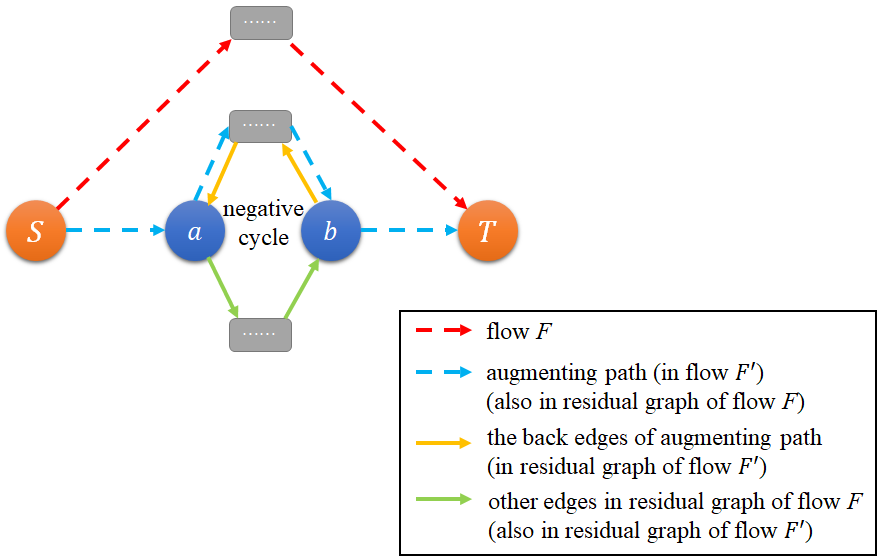
\includegraphics[width=3.3in]{pics/prob3-3.png}\\
      \caption{A negative cycle in the residual graph of flow $F'$} \label{fig3-3}
    \end{figure}

    Hence, the newpath $s \stackrel{F'}{\rightsquigarrow} a \stackrel{r(F')}{\rightsquigarrow} b \stackrel{F'}{\rightsquigarrow} t$ is shorter than path $s \stackrel{F'}{\rightsquigarrow} a \stackrel{F'}{\rightsquigarrow} b \stackrel{F'}{\rightsquigarrow} t$, which contradicts the premise that path $s \stackrel{F'}{\rightsquigarrow} a \stackrel{F'}{\rightsquigarrow} b \stackrel{F'}{\rightsquigarrow} t$ is the shortest path from $s$ to $t$. Therefore, the residual graph of $F'$ still does not contain a negative circle, which completes the induction step.

    In summary, during the construction process of the max flow $F^*$ in our algorithm, there is no negative cycle in the residual graph of the current flow $F$.
    \end{proof}

    \begin{theorem} \label{theorem4}
    The result flow $F^*$ is actually a Minimum Cost Maximum Flow.
    \end{theorem}
    \begin{proof}
    According to Lemma \ref{lemma2}, $F^*$ is the max flow of network $G$.

    According to Lemma \ref{lemma3}, there is no cycle in the residual graph of $F^*$. Then according to Lemma \ref{lemma1}, $F^*$ is the minimum cost flow of the given value $v(F^*)$, which is the max flow value.

    Therefore, $F^*$ is actually a Minimum Cost Maximum Flow.
    \end{proof}

    \begin{solution}
    Theorem \ref{theorem4} give the correctness proof of the algorithm, and Lemma \ref{lemma2} tells us the process can terminates after finding a finite number of augmenting paths. Therefore, the algorithm is correct. Since the residual graph contains negative edge, we must either use the method of Johnson's algorithm to re-weight the edges and use Dijkstra algorithm to calculate the shortest path, or use Bellman-Ford algorithm to calculate the shortest path.

    We can use the distances $dis(u)$ calculated by the Dijkstra algorithm last time to update the potential values $\Phi(u)$ of each vertex. And the re-weight equations of each edge is as follows.
    \begin{displaymath}
    a'(u, v) = a(u, v) + \Phi(u) - \Phi(v)
    \end{displaymath}

    Here are some discussions.
    \begin{itemize}
    \item For the new back edges $(v, u)$, we must have $dis(u) + a(u, v) = dis(v)$ because it is in the shortest path. Therefore,
    \begin{displaymath}
    a'(v, u) = a(v, u) + \Phi(v) - \Phi(u) = -a(u, v) - dis(u) + dis(v) = 0
    \end{displaymath}
    \item For those edge $(u, v)$ that are not affected, we must have $dis(u) + a(u,v) \geq dis(v)$ according to the Triangle Inequality. Therefore,
    \begin{displaymath}
    a'(u, v) = a(u, v) + \Phi(u) - \Phi(v) = a(u, v) + dis(u) - dis(v) \geq 0
    \end{displaymath}
    \end{itemize}

    Therefore, all the costs are non-negative and we can use Dijkstra algorithm to find the shortest path, instead of Bellman-Ford algorithm.

    The implementation of the algorithm is in \href{code/MCMF.cpp}{code/MCMF.cpp}. We also provide another version of implementation, which uses Bellman-Ford algorithm instead of re-weighting and the Dijkstra algorithm, and it is in \href{code/MCMF-BellmanFord.cpp}{code/MCMF-BellmanFord.cpp}. Both of them gives us the answer of the input data in ``MCMF.in'', which is displayed as follows.
    \begin{lstlisting}
Max Flow = 14098
Min Cost (under max flow) = 5290116
    \end{lstlisting}
    Therefore, 
    \begin{itemize}
    \item Max flow = 14098;
    \item Minimum Cost of Max Flow = 5290116.
    \end{itemize}
    \end{solution}


\textbf{Remark:} The source code \emph{SCC.cpp}, and the input data \emph{SCC.in} and \emph{MCMF.in} are attached on the course webpage. Please include your .pdf, .tex, .cpp files for uploading with standard file names.
\end{enumerate}






%========================================================================
\end{document}
